\section*{Korelační přijímač}

Korelační přijímač dále DEM2 provádí korelaci vstupního signálu s bázovými signály, ty odpovídají harmonickým signálům $1,2~kHz$ a $2,2~kHz$. Navíc pro každý z kmitočtů jsou vytvořeny rovnou dva bázové signály posunuté o $\frac{\pi}{2}$. To je kvůli tomu aby korelace měla dostatečnou hodnotu pro libovolnou počáteční fázi. Kvadráty odpovídajících korelací jsou dále sečteny a filtrovány dolní propustí. Tímto postupem získám dva signály det$_1$ a det$_2$, ty jsou nakonec porovnány, čím získáme binární signál.

\begin{figure}[H]
    \centering
    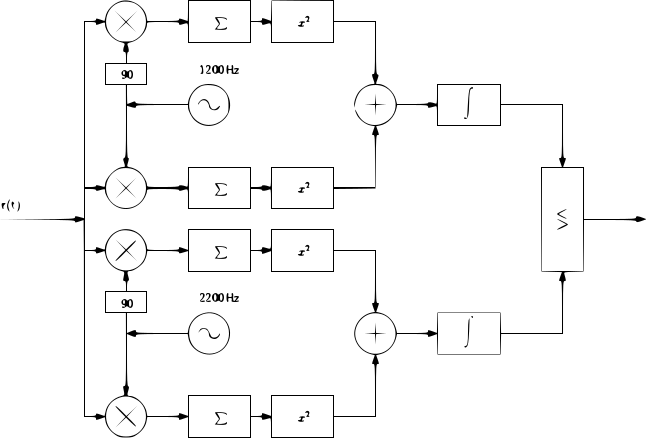
\includegraphics[width=\textwidth]{img/dem2.pdf}
    \caption{Blokové schéma demodulátoru s korelátorem}
\end{figure}

\begin{figure}[H]
    \centering
    \includegraphics[width=0.8\textwidth]{img/base.pdf}
    \caption{Bázové funkce pro korelátor}
\end{figure}

\begin{figure}[H]
    \centering
    \includegraphics[width=0.8\textwidth]{img/cor.pdf}
    \caption{Korelace vstupního signálu s bázovými funkcemi, barvy odpovídají bázovým funkcím}
\end{figure}

\begin{figure}[H]
    \centering
    \includegraphics[width=0.7\textwidth]{img/cor_sum.pdf}
    \caption{Součty kvadrátů odpovídajících bázových funkcí ($\sin$ a $\cos$ stejné frekvence)}
\end{figure}

\begin{figure}[H]
    \centering
    \includegraphics[width=0.7\textwidth]{img/dem2_graph.pdf}
    \caption{Časové průběhy výstupů detektoru a získaného binárního signálu}
\end{figure}